\subsection{Analysis Setup}

\subsubsection{Correlation Analysis Approach}
The central aim of the correlation analysis is to better understand how individual industries relate to the overall dynamics of the manufacturing sector. In particular, we address two guiding research questions. First, we ask whether there is a systematic \textit{lead/lag structure} between industry-level indicators and the main manufacturing index. Identifying such structures would reveal which industries tend to anticipate movements in the aggregate climate and which instead follow with a delay. Second, we investigate whether it is possible to identify \textit{stable subsets of industries} that, across different survey questions and time windows, consistently capture the evolution of the main index. The existence of such subsets would suggest that certain industries carry disproportionate informational value for monitoring the business cycle.

To answer these questions, we adopt a multi-step approach. We begin with a set of \textit{full-sample and rolling window analyses} to estimate correlations between industry-specific indicators and the main index over time. This allows us to detect both long-term structural relationships and short-term temporal fluctuations. Next, we apply a \textit{ranking-based consensus analysis}, which tracks how the relative importance of industries changes across questions and windows. This step provides a way to monitor stability and detect re-orderings in the correlation structure. Finally, we develop a \textit{scoring model} that integrates information across time and questions in order to identify those industries that remain consistently close to the main index. Taken together, these steps provide a framework for moving beyond one-off correlation estimates towards a systematic evaluation of persistence, stability, and cross-question robustness.

The focus throughout is on correlations between the survey’s main manufacturing index and the industry-level indicators. All industry codes are analyzed individually, and we highlight industries whose correlations are either particularly strong or reveal distinctive lead/lag patterns. These industries are of special interest as they may function as early-warning signals or as anchors for constructing composite indicators.

\subsubsection{Data Structure}
The structure of the underlying data introduces important considerations for the correlation analysis. Industry codes are distributed unequally across sectors and hierarchical levels, as illustrated in Figure~\ref{fig:industries_by_sector}. This imbalance has non-trivial effects: rather than distorting results, the over-representation of certain sectors appears to \textit{reinforce} the observed correlation structure. In particular, retaining the natural weighting implied by the hierarchy yields stronger and more coherent correlations between industry-level indicators and the main question than alternative approaches where correlations are first aggregated within sectors (e.g., by mean or median) and then averaged across sector values. 

\begin{figure}[H]
    \centering
    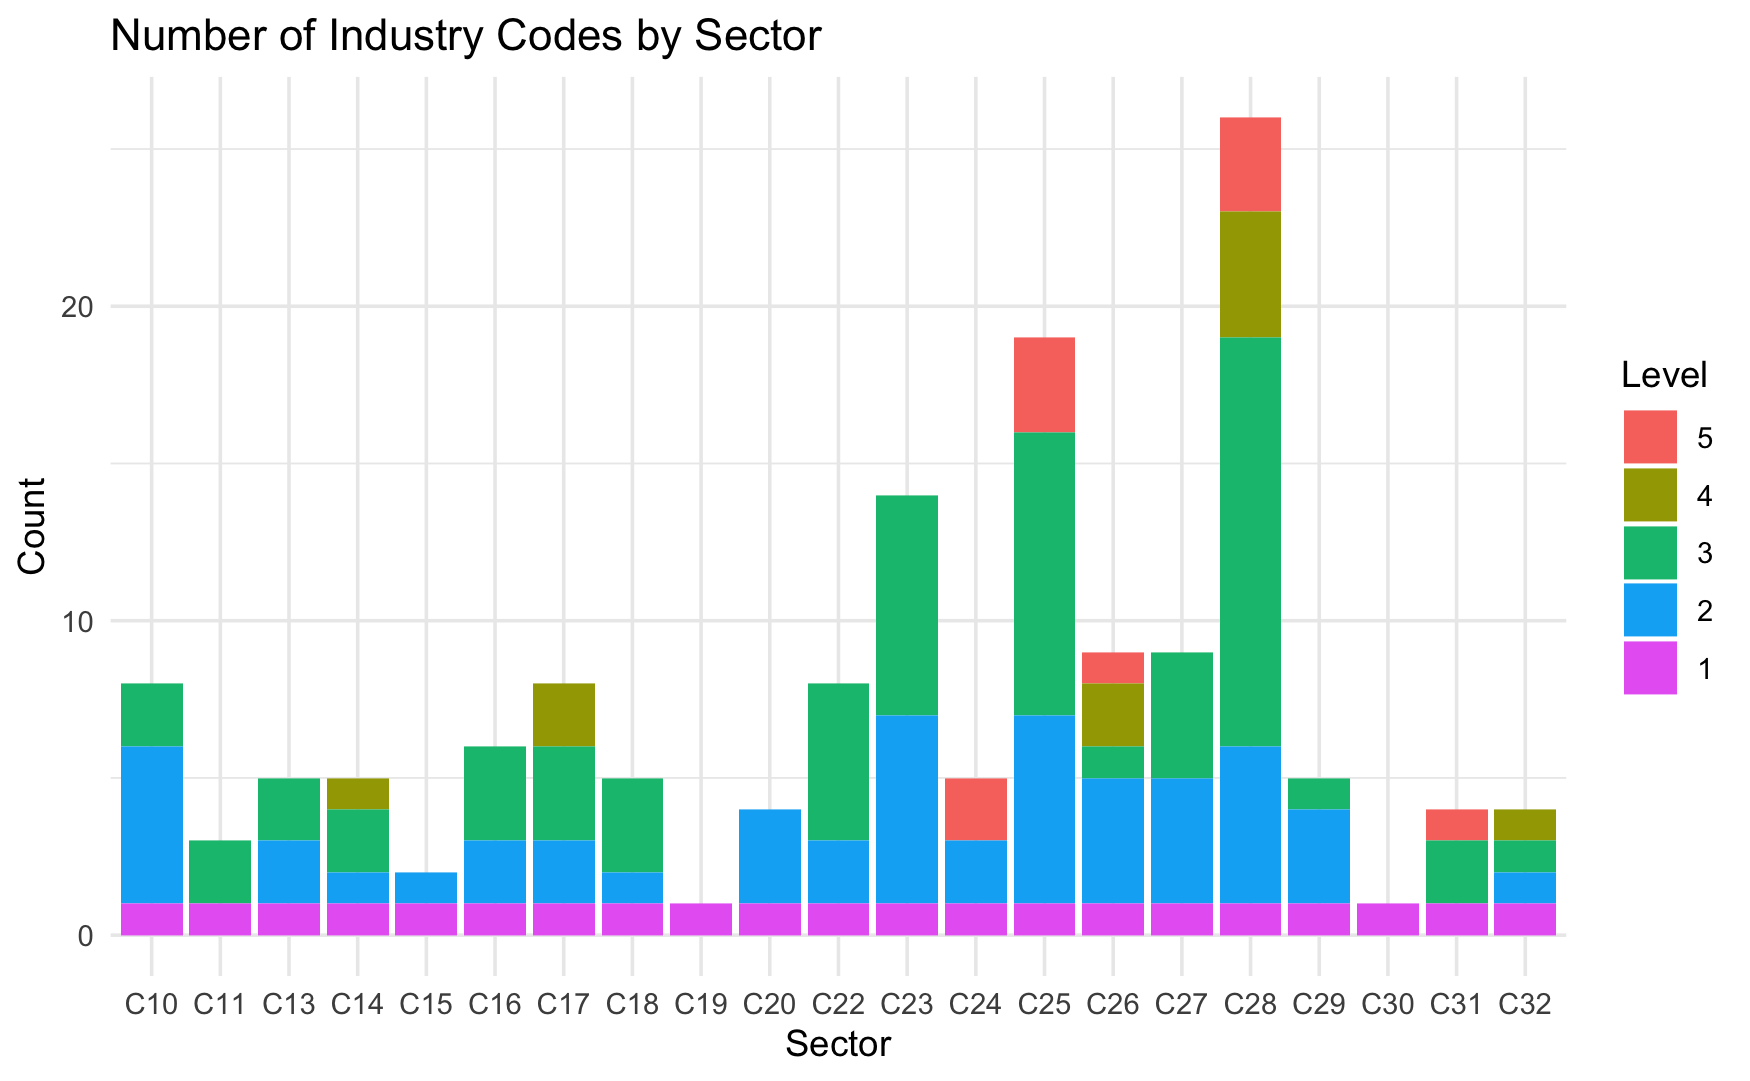
\includegraphics[width=0.7\linewidth]{DominikPlots/as_industries_by_sector.png}
    \caption{Number of industry codes by sector and hierarchical level.}
    \label{fig:industries_by_sector}
\end{figure}

This observation suggests that the hierarchical design of the industry codes reflects genuine structural dependencies in the data. For this reason, levels 4--5 of the hierarchy, which contain relatively sparse numbers of codes, are analyzed separately to avoid dilution effects. An overview of the manufacturing sectors included in the survey is provided in Table~\ref{tab:sectors}, while Figure~\ref{fig:industries_by_sector} summarizes the distribution of industry codes across sectors and levels.



\subsubsection{Stationarity}
\label{stationarity}
Stationarity of indices is often regarded as a prerequisite for correlation analysis, since the presence of common trends can artificially inflate correlations by introducing dependence driven by trend alone.  

In our dataset, however, not all industry codes are stationary. As illustrated in Figure~\ref{fig:comparison_earlypred_profiles}, many industry codes show a stationary KLD index over time. Yet if we required full stationarity across all questions and time windows, no industry code would satisfy this condition.  

\begin{figure}[H]
    \centering
    \begin{subfigure}[t]{0.48\linewidth}
        \centering
        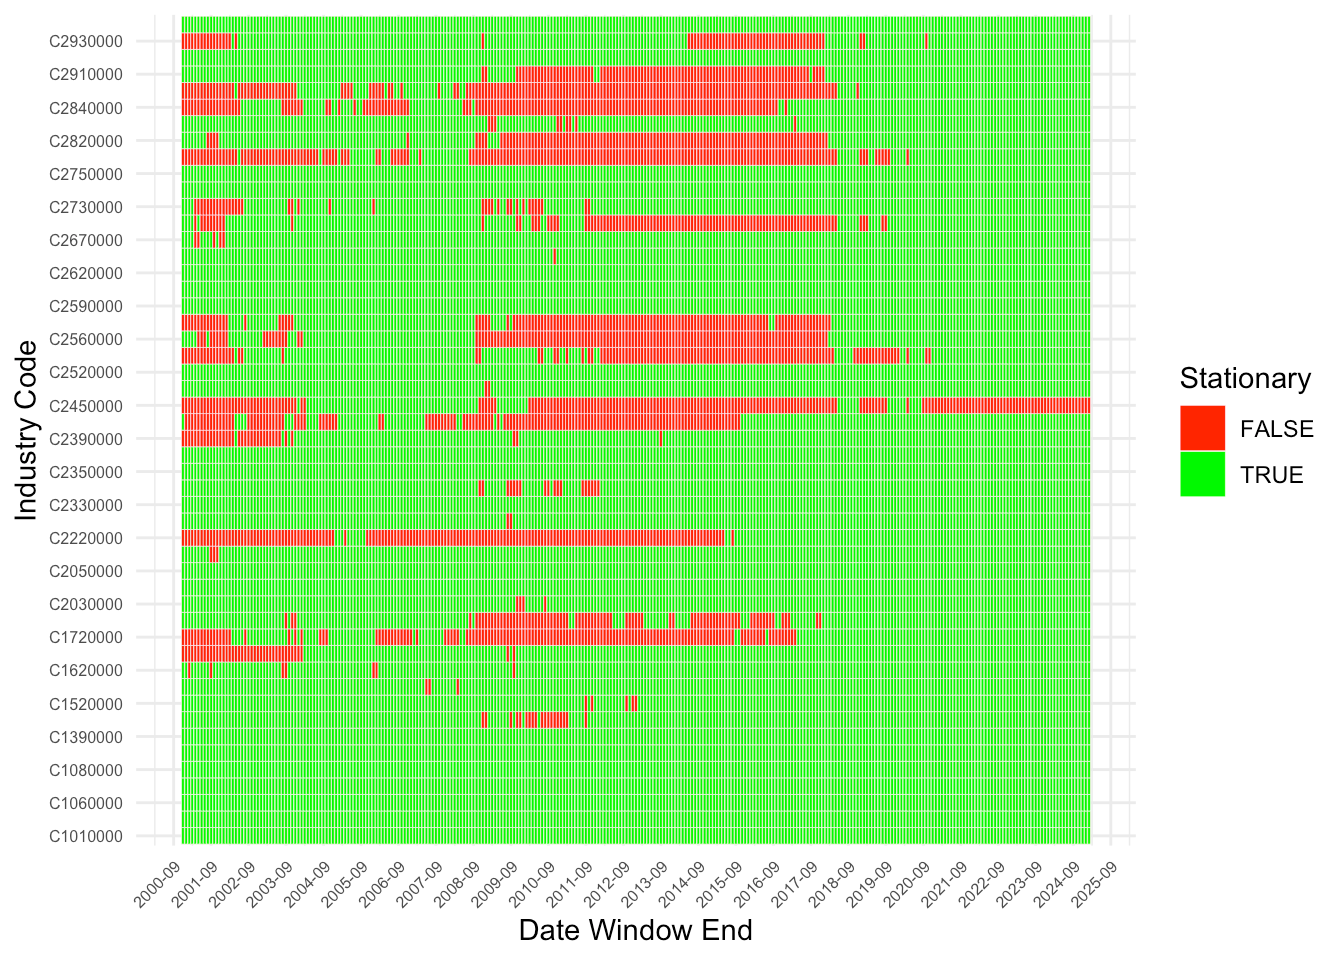
\includegraphics[width=\linewidth]{DominikPlots/as_stat_kld.png}
        \caption{Stationary industries (KLD).}
        \label{fig:stat_kld}
    \end{subfigure}%
    \hfill
    \begin{subfigure}[t]{0.48\linewidth}
        \centering
        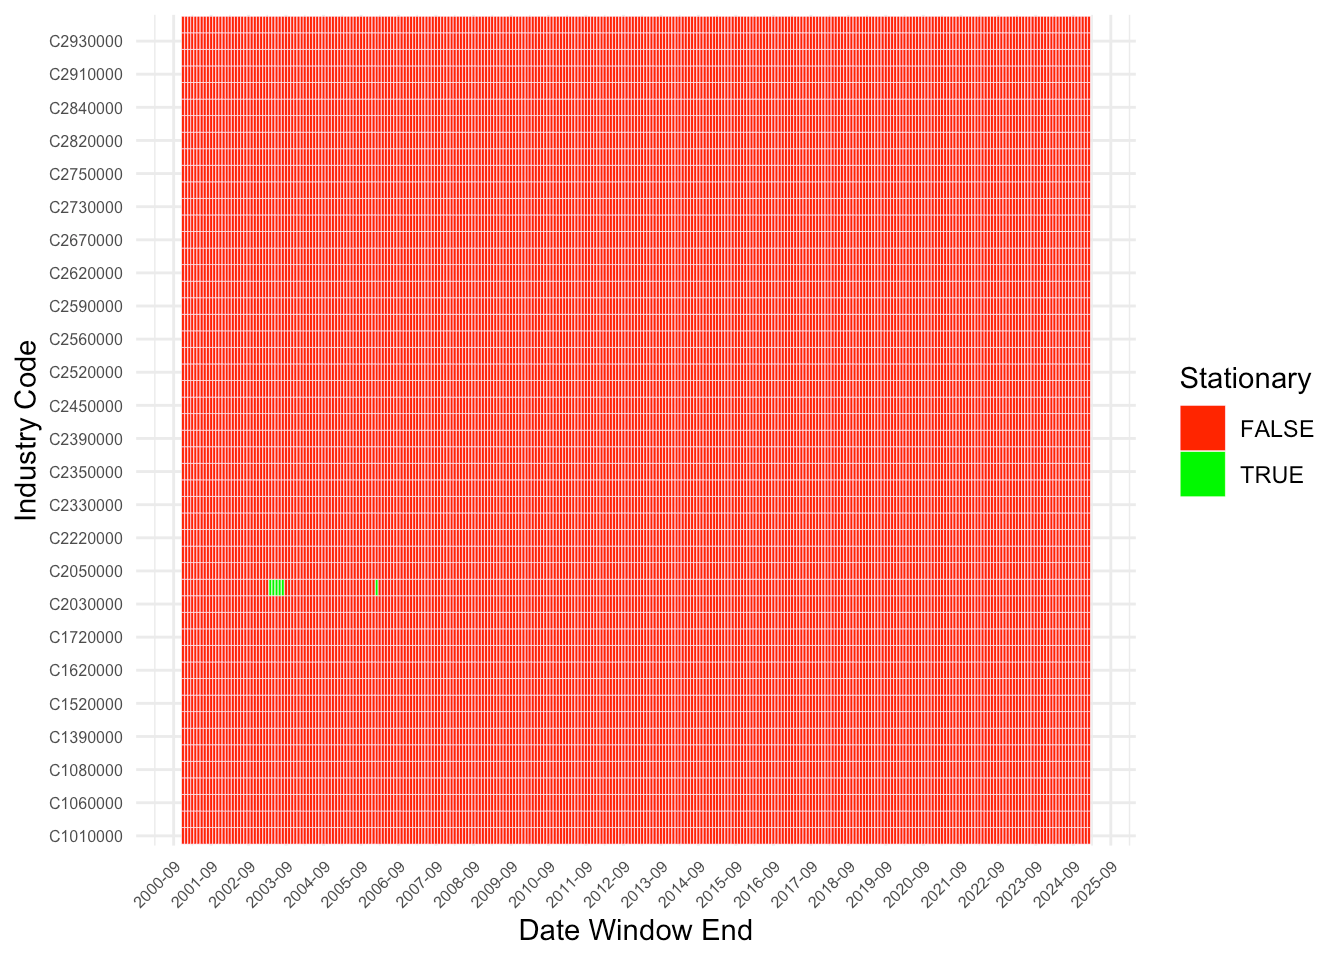
\includegraphics[width=\linewidth]{DominikPlots/as_stat_overall.png}
        \caption{Stationary industries (all questions).}
        \label{fig:stat_overall}
    \end{subfigure}
    \caption{Comparison of stationarity across time windows and questions.}
    \label{fig:comparison_earlypred_profiles}
\end{figure}

For the purposes of this study, we therefore did not impose stationarity as a strict requirement. While stationarity is generally desirable, excluding non-stationary series would eliminate too much information. Allowing for non-stationary indices may lead to higher measured correlations compared to the strict statistical definition, but in an economic context this is not necessarily problematic. In fact, when trends dominate certain rolling windows, correlations in trend may represent economically meaningful co-movement. From this perspective, we do not distinguish between ``true'' correlation and correlation driven by shared trends, as both can provide valuable insights into cyclical dynamics.  



\subsubsection{Correlation Metrics}
To quantify the relationship between industry-level indicators and the main manufacturing index, we employ two complementary measures: \textit{cross-correlation} and \textit{distance correlation}. Using both metrics allows us to balance interpretability with sensitivity to nonlinear dependencies.

\vspace{\baselineskip}
\textbf{Cross-correlation:}  
Cross-correlation, implemented via \texttt{stats::ccf}, measures the linear association between two time series at different leads and lags. It provides both the direction and magnitude of potential lead--lag structures. Because of its direct interpretability in terms of timing and sign, cross-correlation serves as the primary tool for detecting industries that anticipate or follow the dynamics of the main index.

\vspace{\baselineskip}
\textbf{Distance correlation:}  
Distance correlation, implemented via \texttt{energy::dcor}, extends beyond linear relationships by detecting any form of statistical dependence, including nonlinear or nonmonotonic structures. A key property of distance correlation is that it equals zero if and only if the variables are independent. In our setting, it thus provides an upper bound relative to linear correlation ($|\rho|$) and signals whether cross-correlation may understate the strength of dependencies. The measure was introduced and studied in detail by \citet{Szekely2007}.

\vspace{\baselineskip}
\vspace{\baselineskip}
Cross-correlation provides an intuitive baseline for interpreting the temporal structure of dependencies. Distance correlation, in turn, validates these findings by checking whether the relationships are predominantly linear or whether nonlinearities play a substantial role. In practice, both metrics yield strikingly similar structures (Figures~\ref{fig:median_ccf} and \ref{fig:median_dcor}), suggesting that linear dependence accounts for the bulk of the observed relationships. Importantly, the combined figures also show that the strongest correlations are concentrated within a window of approximately $\pm 6$ months. The peak correlation for each question consistently lies within this lag range. For this reason, all subsequent analyses focus on lags within $\pm 6$ months, unless explicitly stated otherwise.\footnote{Rolling-window analyses introduced later confirm that this lag structure is stable across time and holds both in normal periods and during major economic disruptions.}

\begin{figure}[H]
    \centering
    \begin{subfigure}[t]{0.48\linewidth}
        \centering
        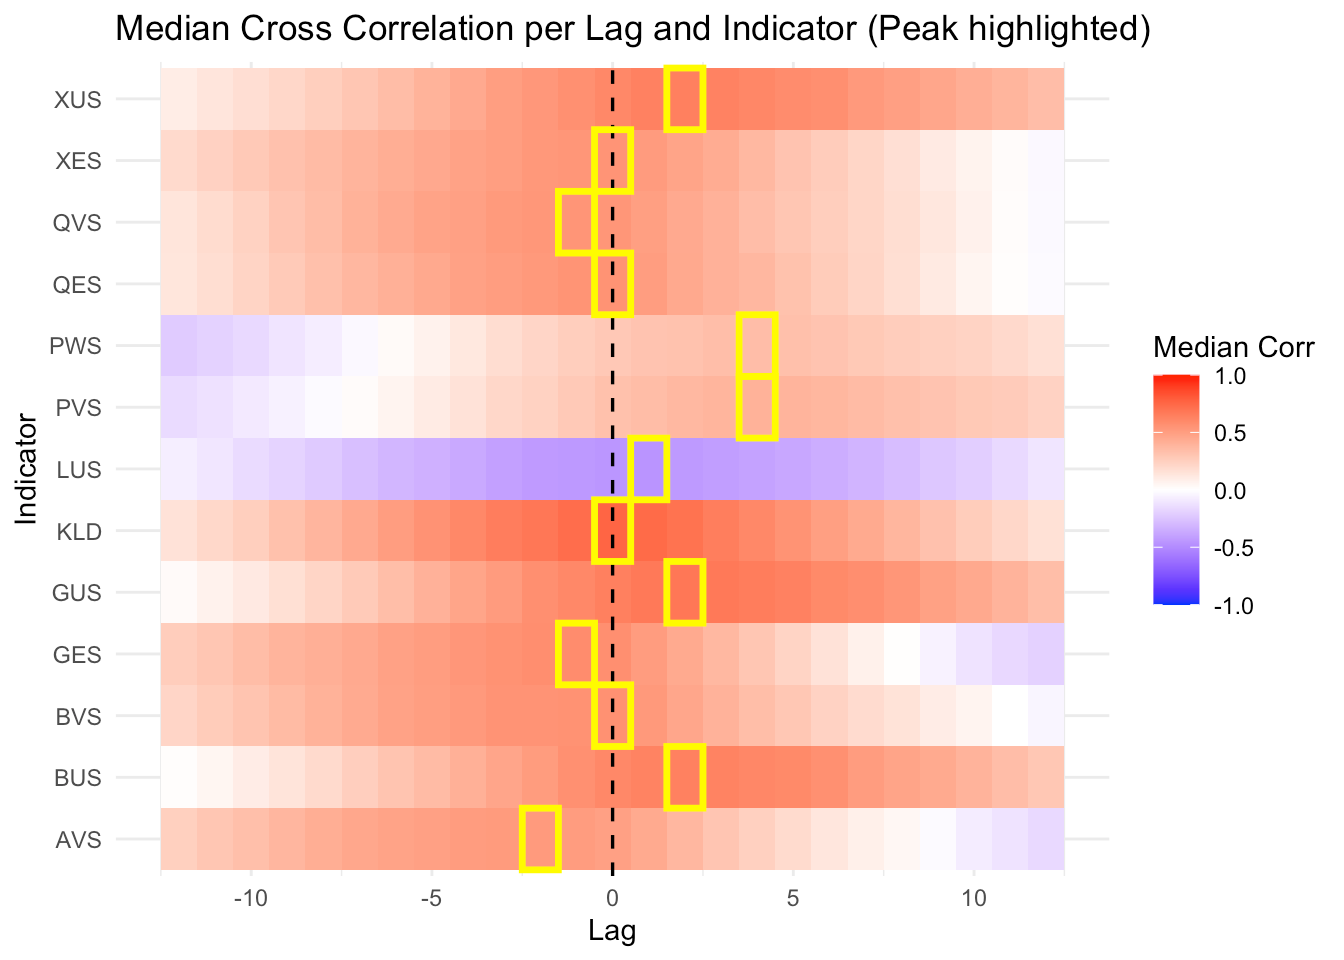
\includegraphics[width=\linewidth]{DominikPlots/as_median_ccf.png}
        \caption{Median cross-correlation profiles across industries.}
        \label{fig:median_ccf}
    \end{subfigure}%
    \hfill
    \begin{subfigure}[t]{0.48\linewidth}
        \centering
        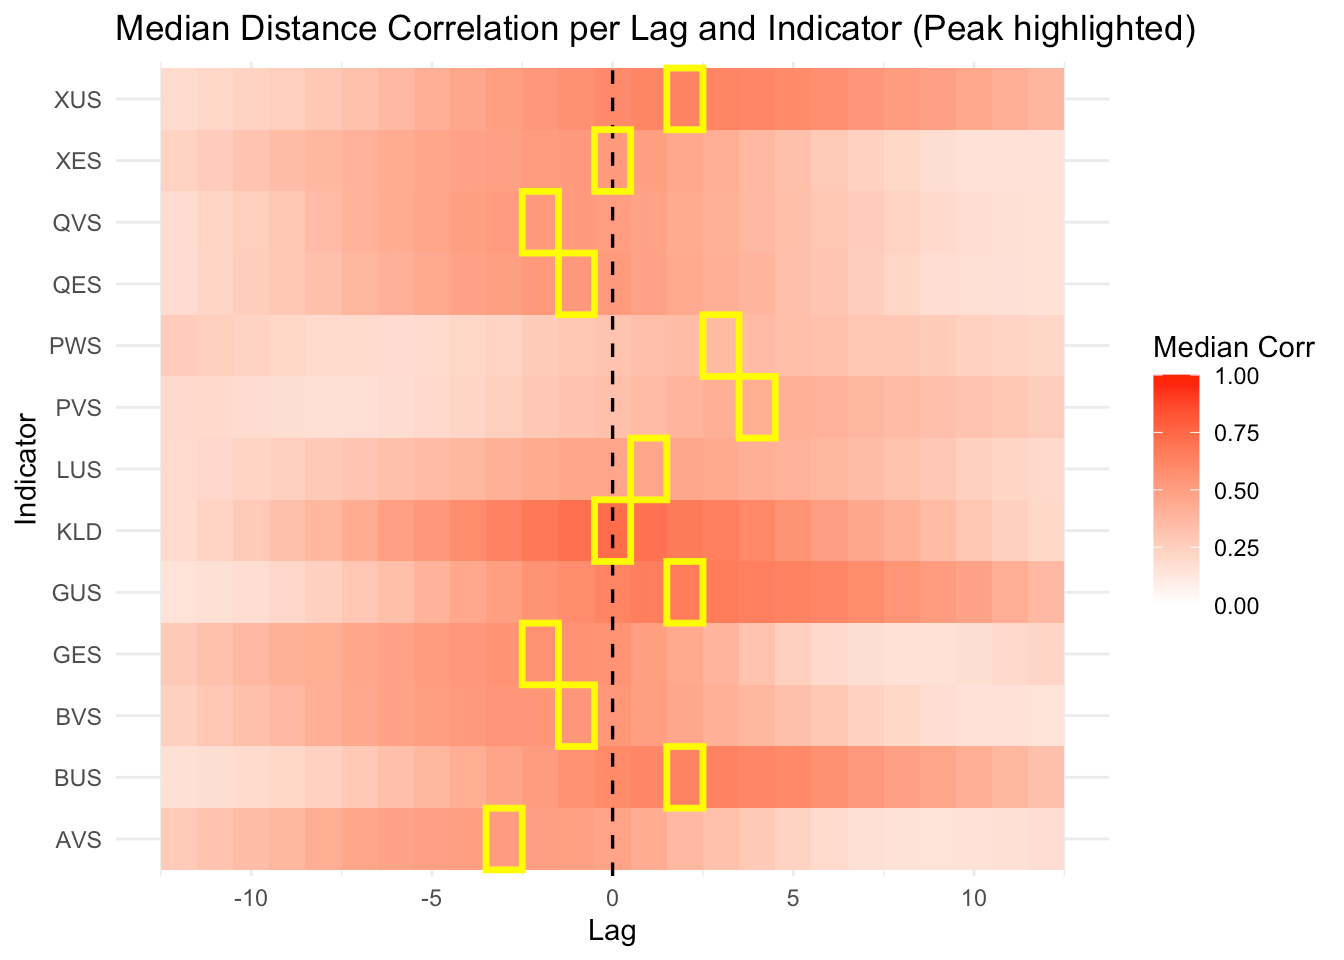
\includegraphics[width=\linewidth]{DominikPlots/as_median_dcor.png}
        \caption{Median distance-correlation profiles across industries.}
        \label{fig:median_dcor}
    \end{subfigure}
    \caption{Comparison of median cross-correlation and distance-correlation profiles across industries.}
    \label{fig:correlation_profiles}
\end{figure}


\subsection{Correlation Distribution}
To gain a deeper understanding of the correlation structure between the survey questions and the main index, we analyze the distribution of correlations at the level of individual questions and industry codes. The goal of this exercise is to disentangle how strongly different industries contribute to the aggregate signal, and how stable these relationships are across time, sectors, and hierarchical levels.

Because the central point of interest here is the \textit{strength of dependence}, we focus on distance correlation as the primary metric. Unlike cross-correlation, which emphasizes timing and direction, distance correlation allows us to summarize the overall magnitude of association independently of linearity or lag alignment. This makes it a natural choice for characterizing the distribution of correlations across a large number of industries.

\subsubsection{Correlation Distribution by Time}
From an economic perspective, it is important to assess whether the correlation structure remains stable across different phases of the business cycle, particularly during downturns and periods of stress compared to times of economic expansion. Figure~\ref{fig:cd_ccf_roll} illustrates how average cross-correlations evolve across rolling windows, highlighting both the mean level and the location of peak lags.

\begin{figure}[H]
    \centering
    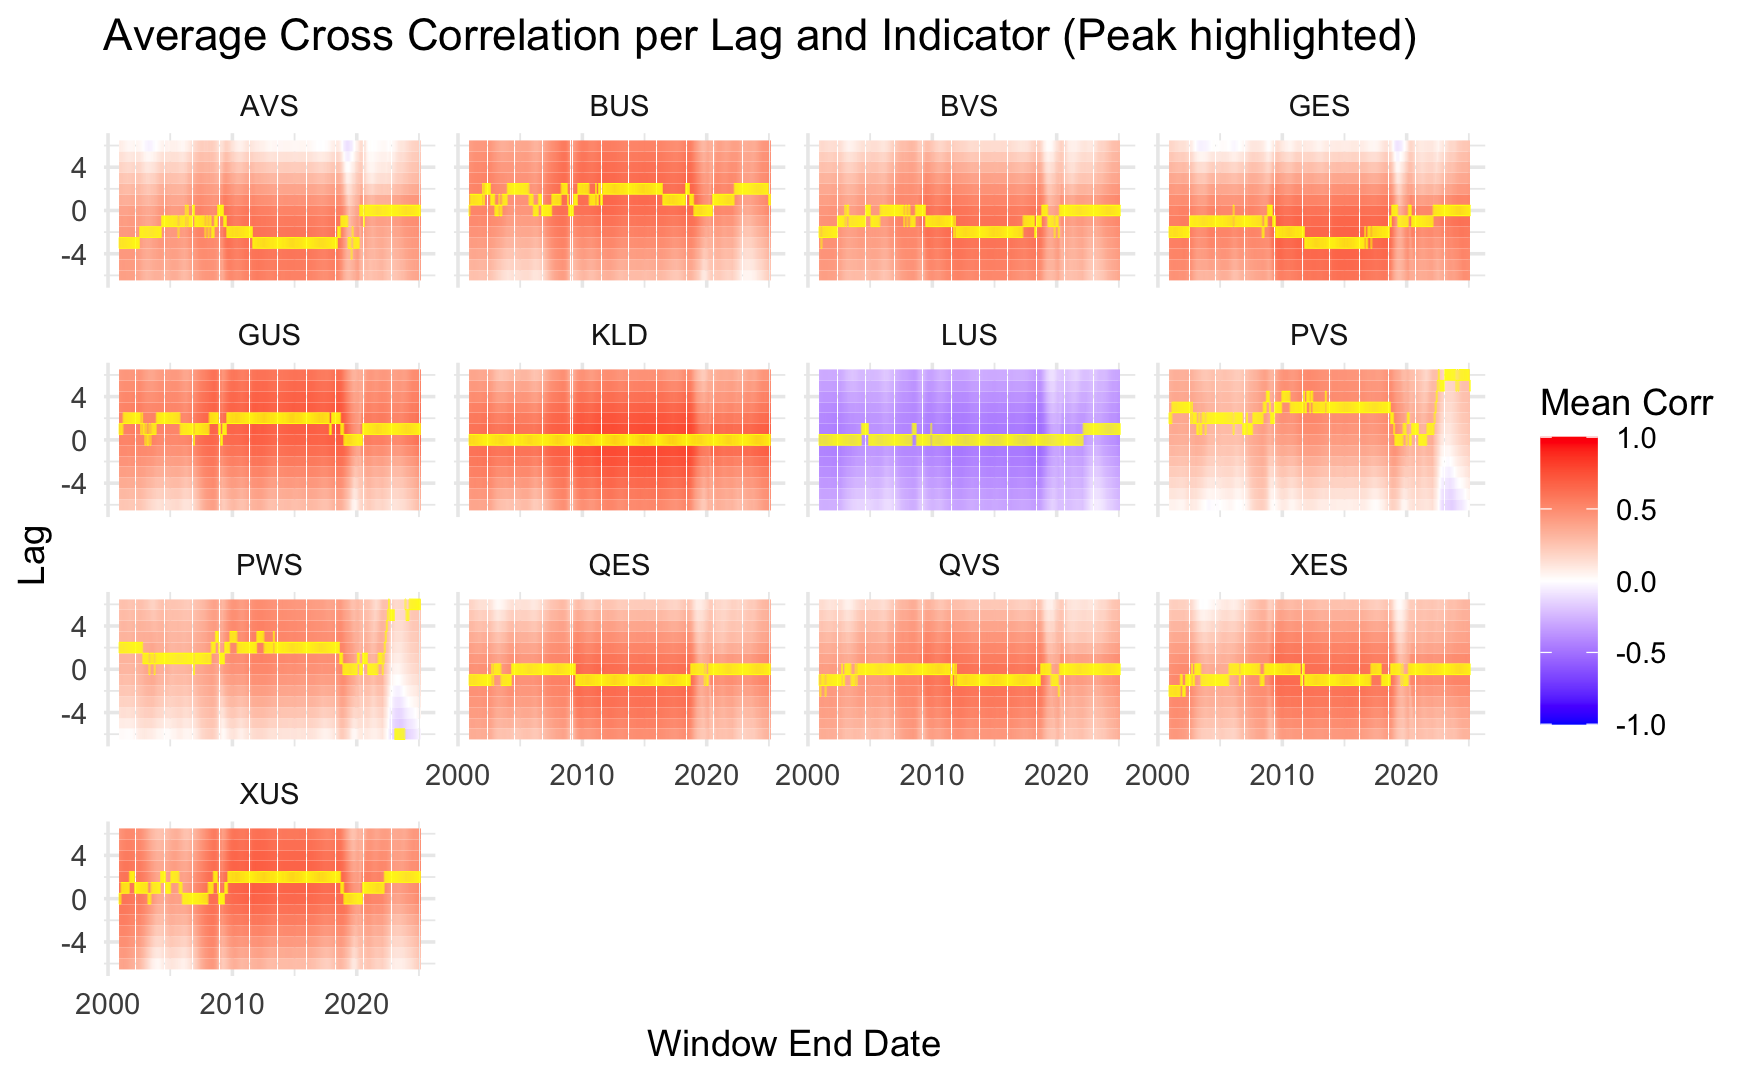
\includegraphics[width=0.7\linewidth]{DominikPlots/cd_ccf_roll.png}
    \caption{10-year rolling window analysis (1-month step), 2000--2025.}
    \label{fig:cd_ccf_roll}
\end{figure}

Beyond average correlations, it is equally important to study the \textit{distribution} of correlations across industries. Figure~\ref{fig:peak_dcor} presents the development of peak distance correlations over time, disaggregated by question. The figure shows both the median (red line) and the dispersion across industry codes (quantiles), thereby capturing not only the central tendency but also the variance of the dependence structure.

\begin{figure}[H]
    \centering
    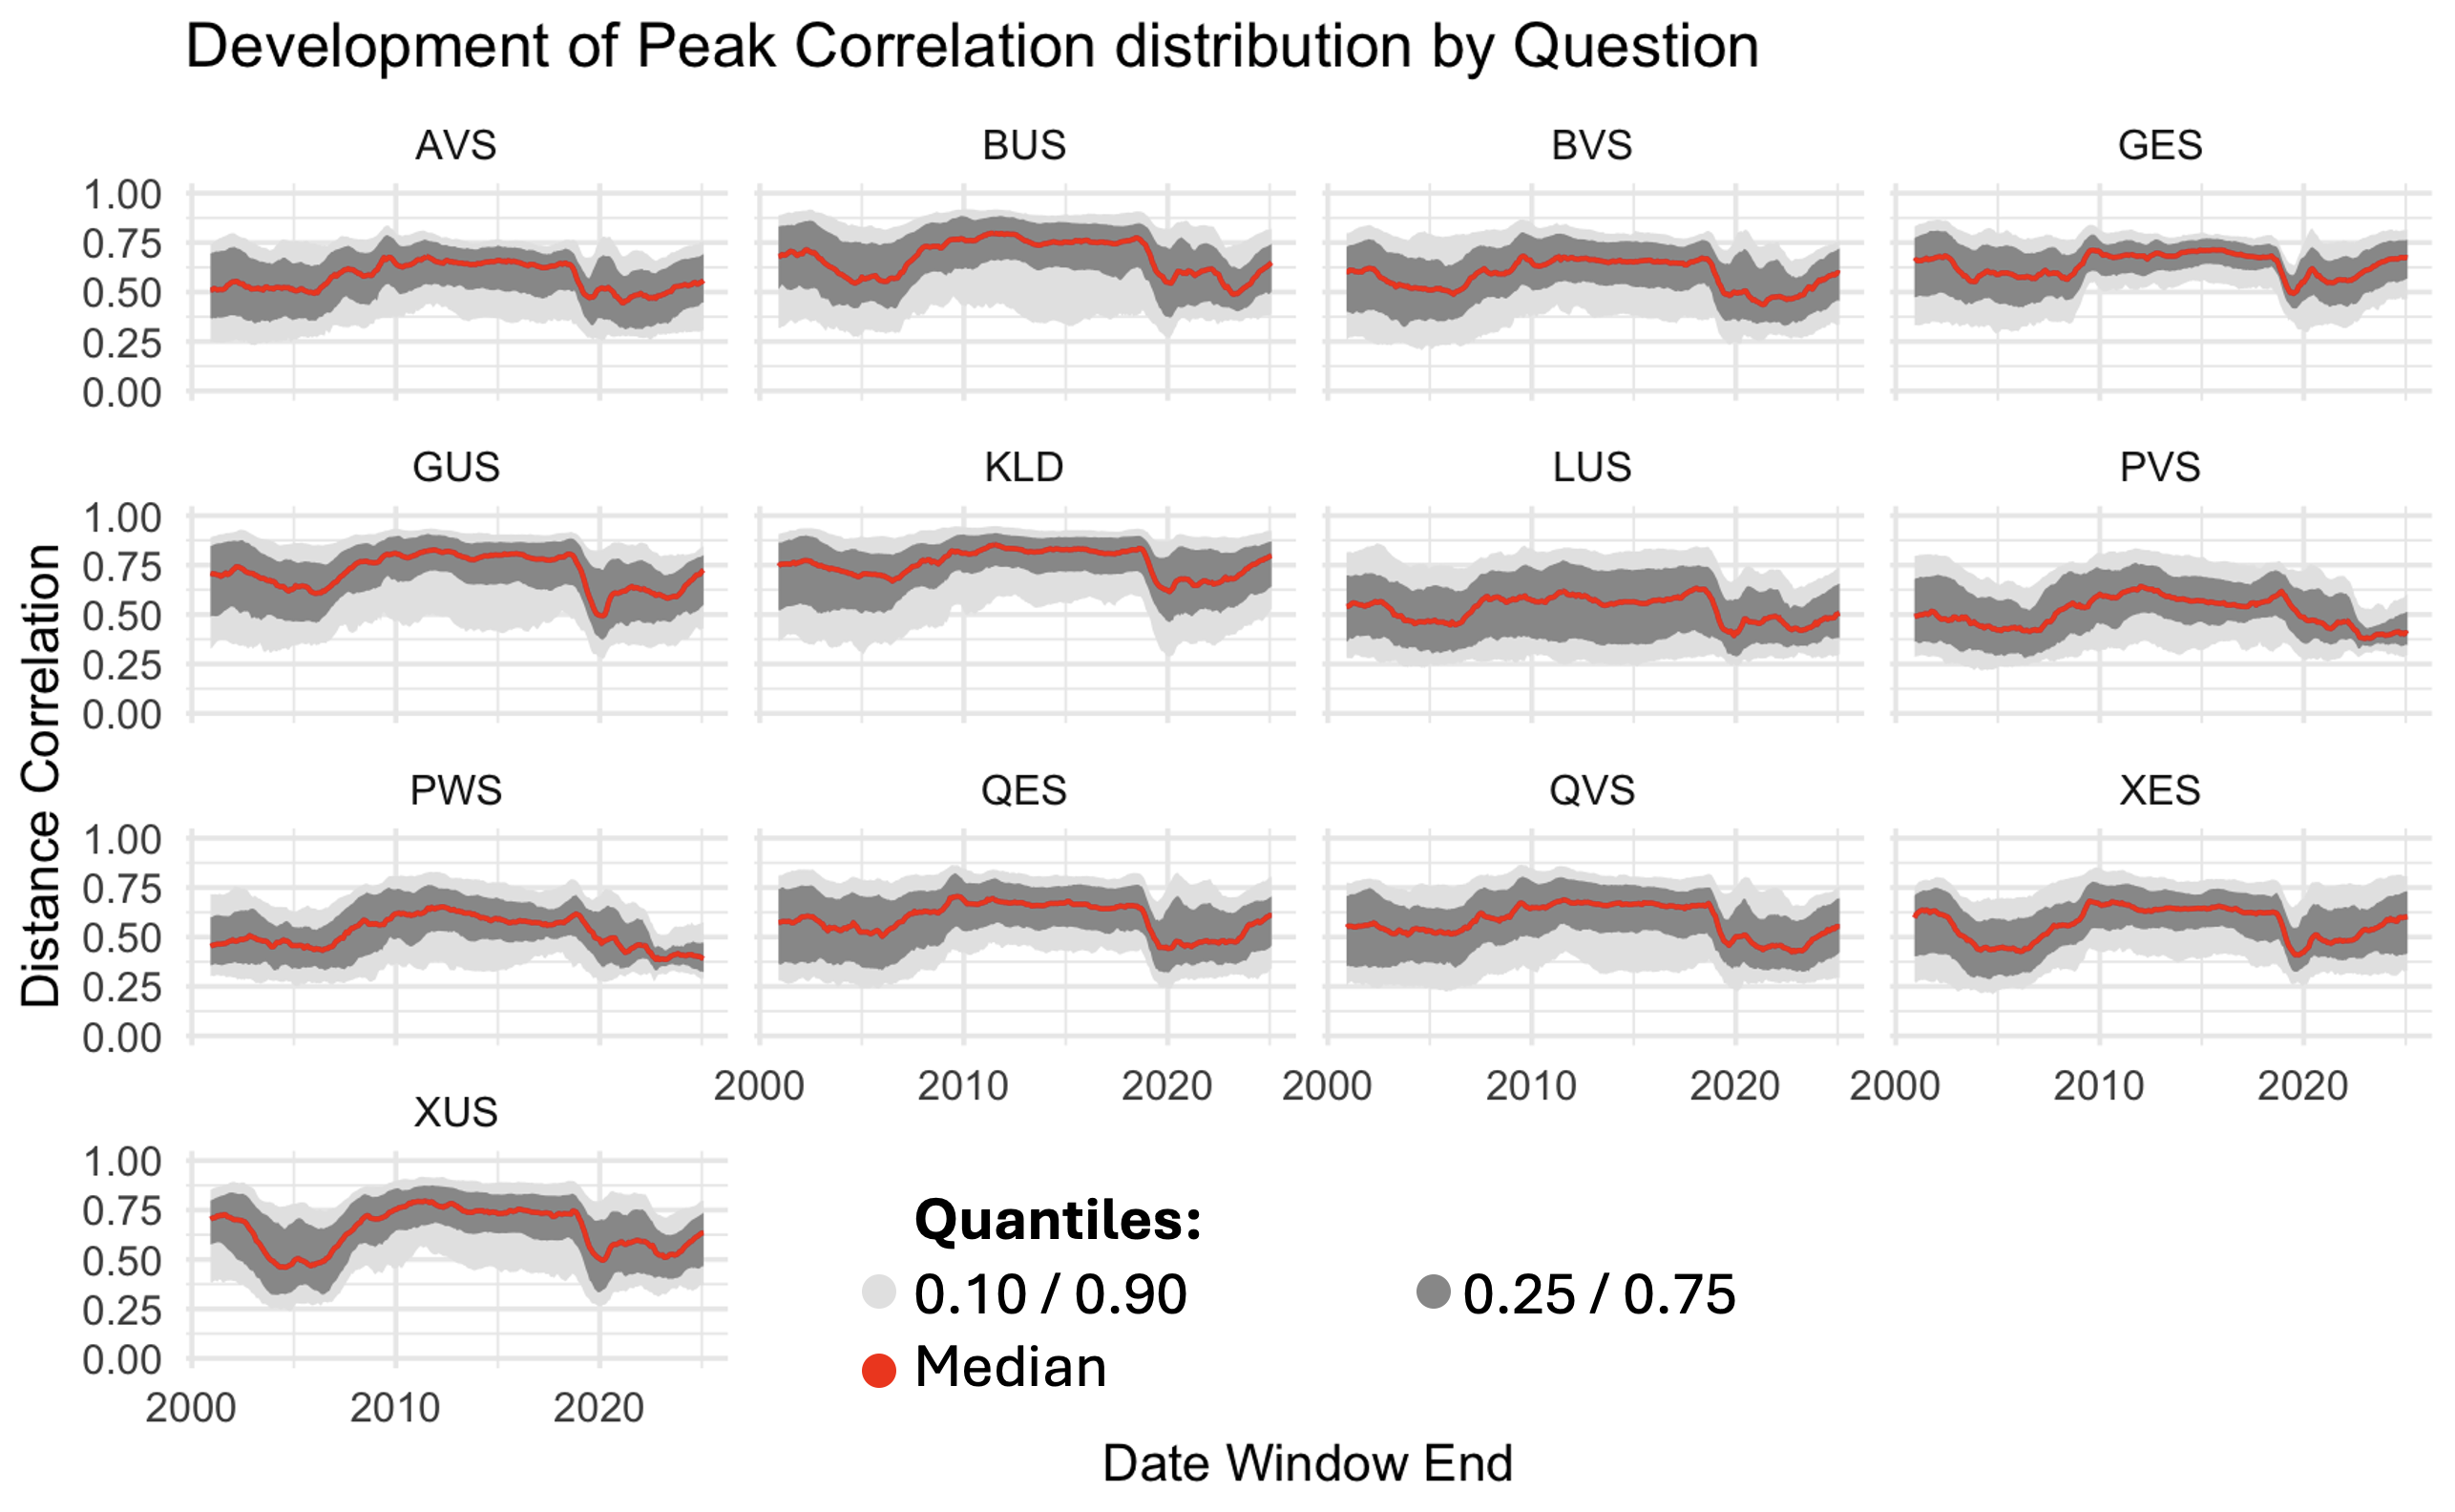
\includegraphics[width=0.7\linewidth]{DominikPlots/cd_dcor_dist_roll.png}
    \caption{Peak distance correlation by question, with median and inter-quantile ranges, Levels 1--3.}
    \label{fig:peak_dcor}
\end{figure}

\vspace{\baselineskip}
\vspace{\baselineskip}
Taken together, these results highlight two important insights. First, the correlation structure exhibits clear breaks around major economic events, most notably the global financial crisis of 2008--2009 and the COVID-19 pandemic after 2018. During these periods, both the level and the dispersion of correlations shift markedly, reflecting heterogeneous responses of industries to systemic shocks. Second, despite these disruptions, the overall correlation structure remains relatively stable in calmer periods, suggesting that the main index captures persistent common dynamics across manufacturing industries. This stability provides reassurance that industry-level correlations can serve as reliable indicators of aggregate developments, while the observed breaks emphasize their usefulness in detecting structural shifts.

\subsubsection{Correlation Distribution by Sector}
Examining the distribution of peak distance correlations at the sector level reveals substantial heterogeneity across industries (Figure~\ref{fig:cd_dcor_dist_sector}). Some sectors exhibit consistently strong correlations with the main index, while others display weaker or more dispersed relationships. This underlines the heterogeneous character of the German manufacturing landscape, where not all industries contribute equally to the aggregate dynamics.

\begin{figure}[H]
    \centering
    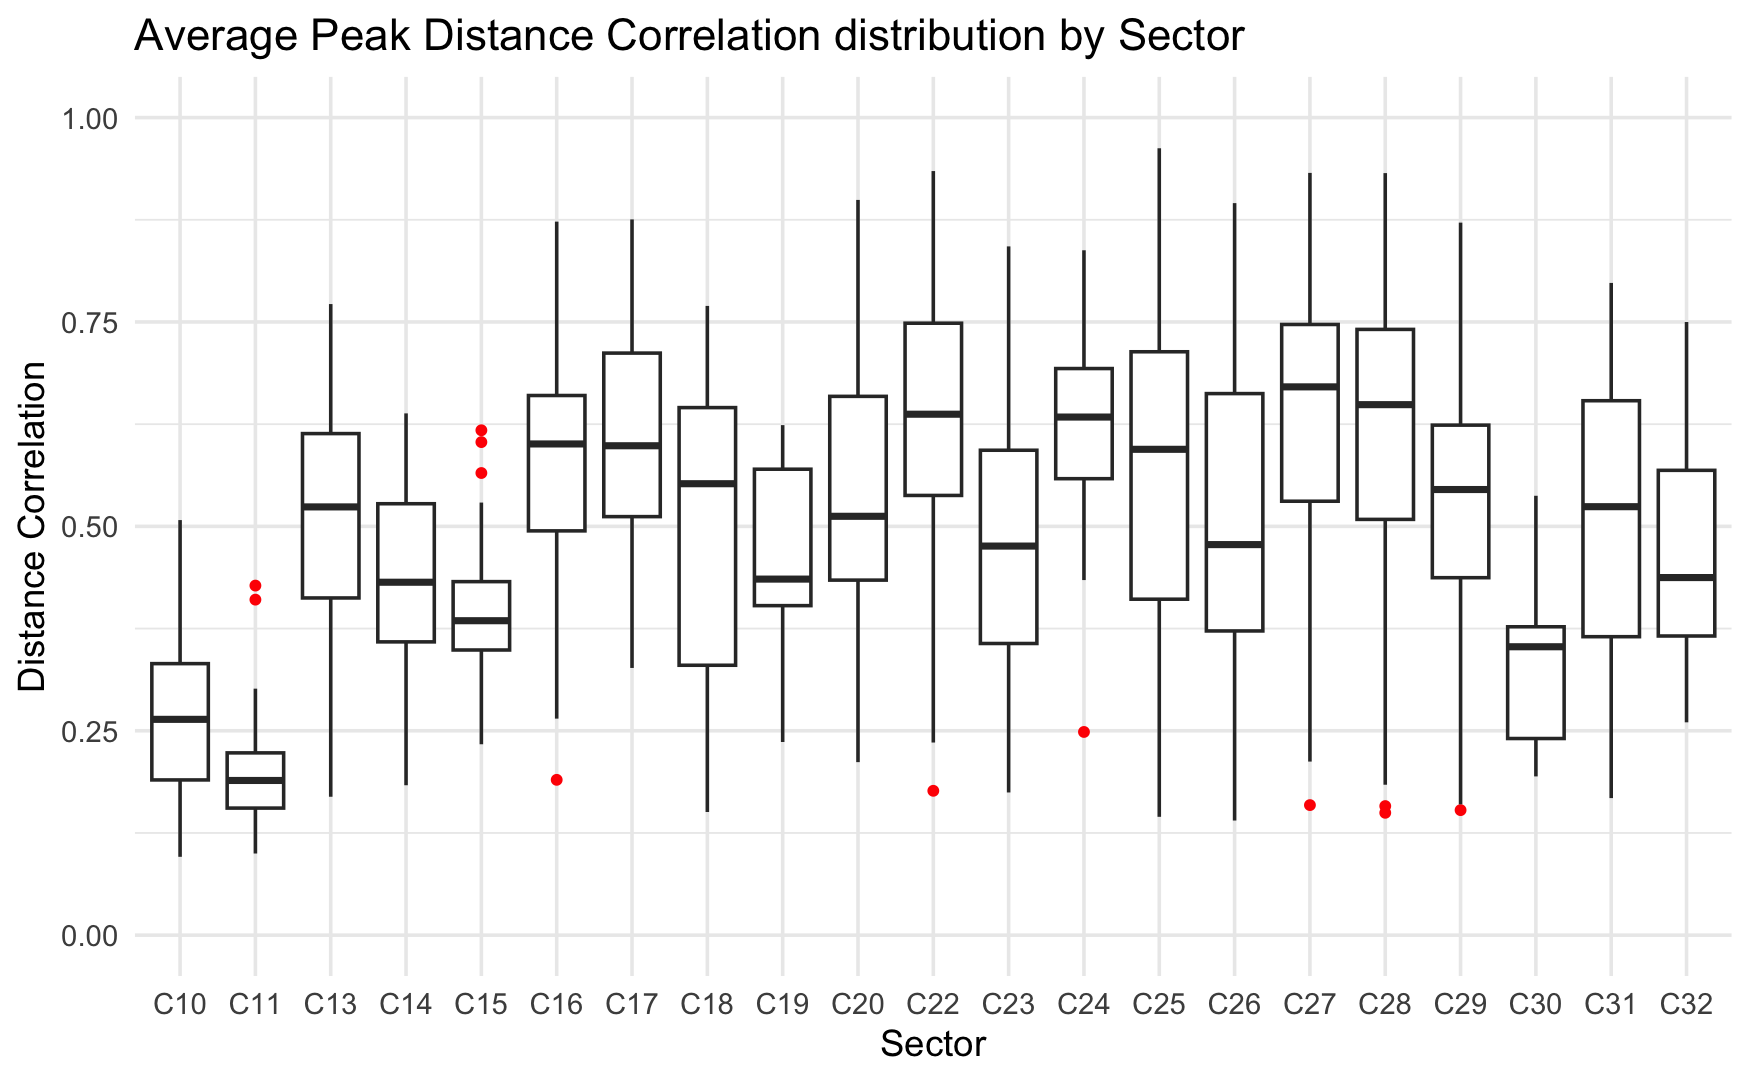
\includegraphics[width=0.7\linewidth]{DominikPlots/cd_dcor_dist_sector.png}
    \caption{Distribution of peak distance correlations by sector.}
    \label{fig:cd_dcor_dist_sector}
\end{figure}

It is important to note that the aggregation underlying the main index is weighted by the economic importance of each sector. As a result, the index successfully reflects overall economic developments, but it does not necessarily mirror the behavior of each individual industry. Certain sectors may therefore play only a limited role in shaping the aggregate signal, even though they are economically relevant in their own right.

From a modeling perspective, these results suggest that the dynamics of the main index can be effectively captured by focusing on a smaller set of industries with consistently strong correlations. Identifying such sectors provides a path towards sparser models that retain explanatory power while avoiding the noise introduced by less strongly aligned industries.


\subsubsection{Correlation Distribution by Level}
As discussed previously, the hierarchical structure of industry codes introduces an inherent imbalance in the number of series across levels. To account for this, we evaluate the correlation distribution separately for the more granular Levels~4--5. Figure~\ref{fig:cd_dcor_dist_level} provides an overview of the distribution of peak distance correlations across levels.

\begin{figure}[H]
    \centering
    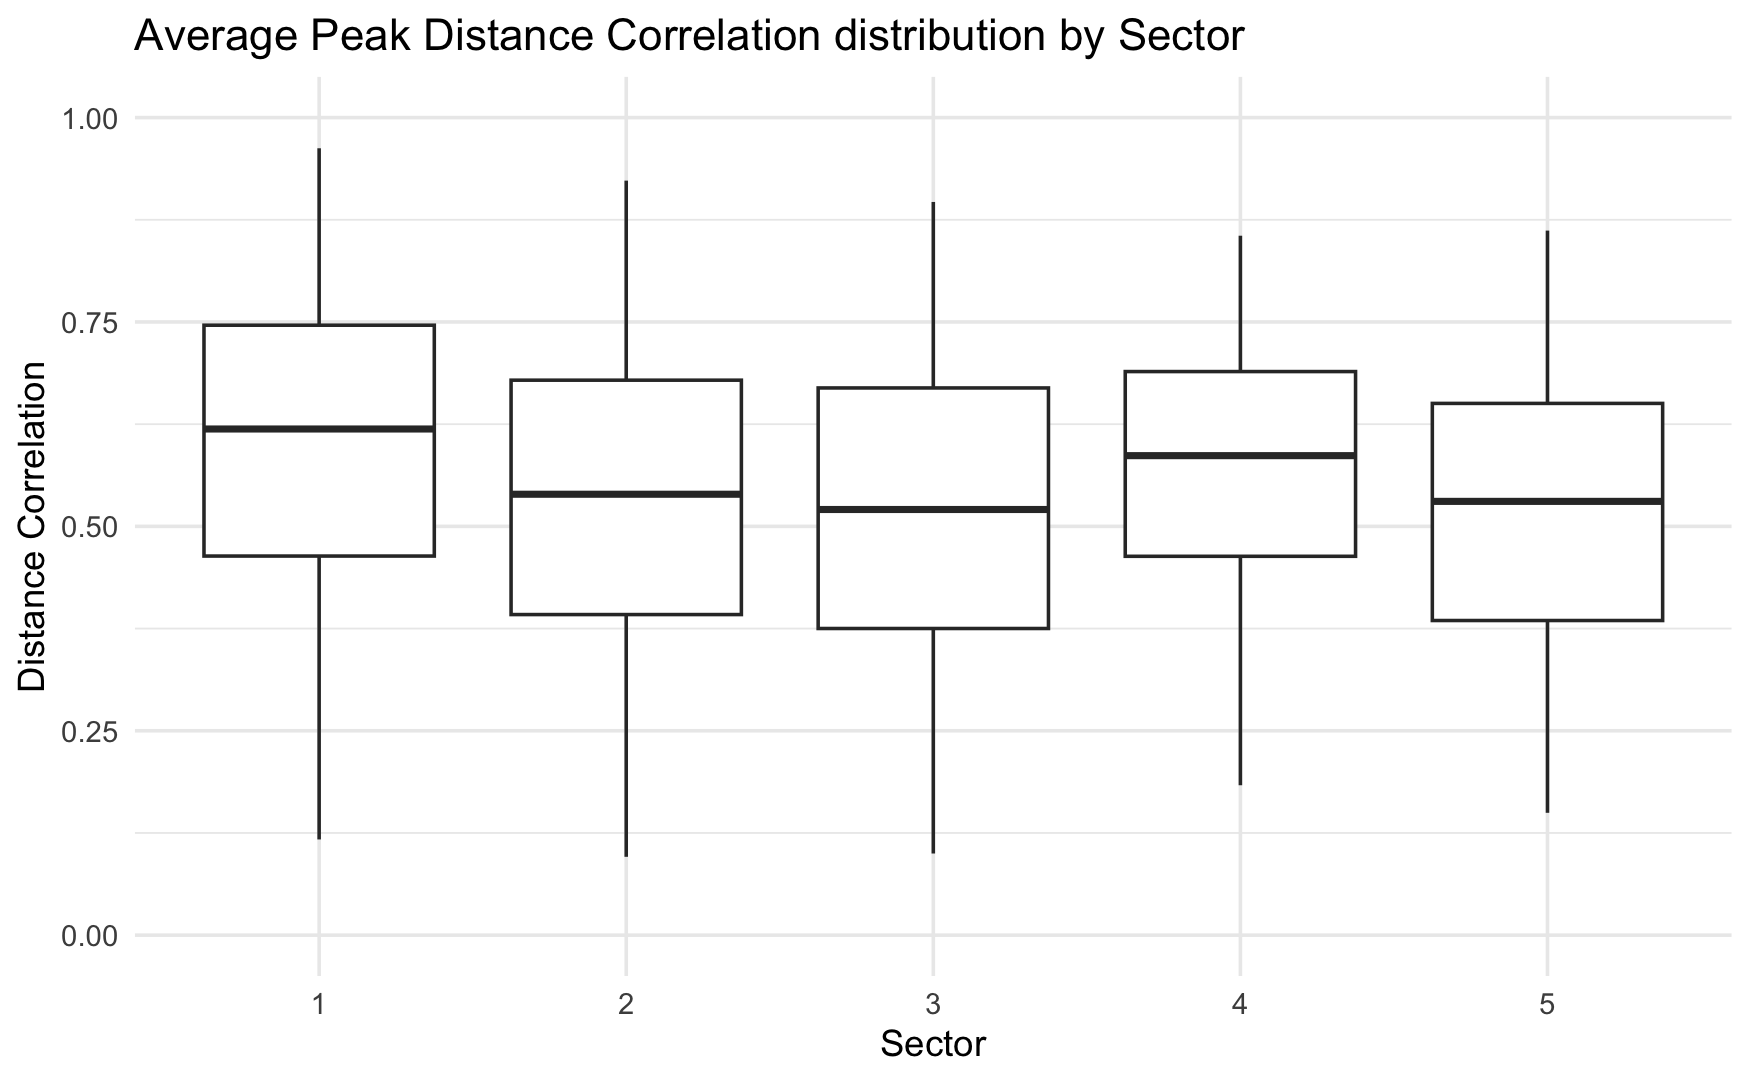
\includegraphics[width=0.7\linewidth]{DominikPlots/cd_dcor_dist_level.png}
    \caption{Distribution of peak distance correlations by hierarchical level.}
    \label{fig:cd_dcor_dist_level}
\end{figure}

The overall picture is that Levels~4--5 exhibit somewhat noisier correlation structures compared to the higher-level aggregations, but they broadly follow the same patterns observed at Levels~1--3. This similarity also extends to their temporal development (Figure~\ref{fig:cd_dcor_dist_roll_level}), where the rolling-window evolution of distance correlations at deeper levels closely tracks that of the broader aggregates. In short, Levels~4--5 appear more volatile, but they remain aligned with the higher-level dynamics.

\begin{figure}[H]
    \centering
    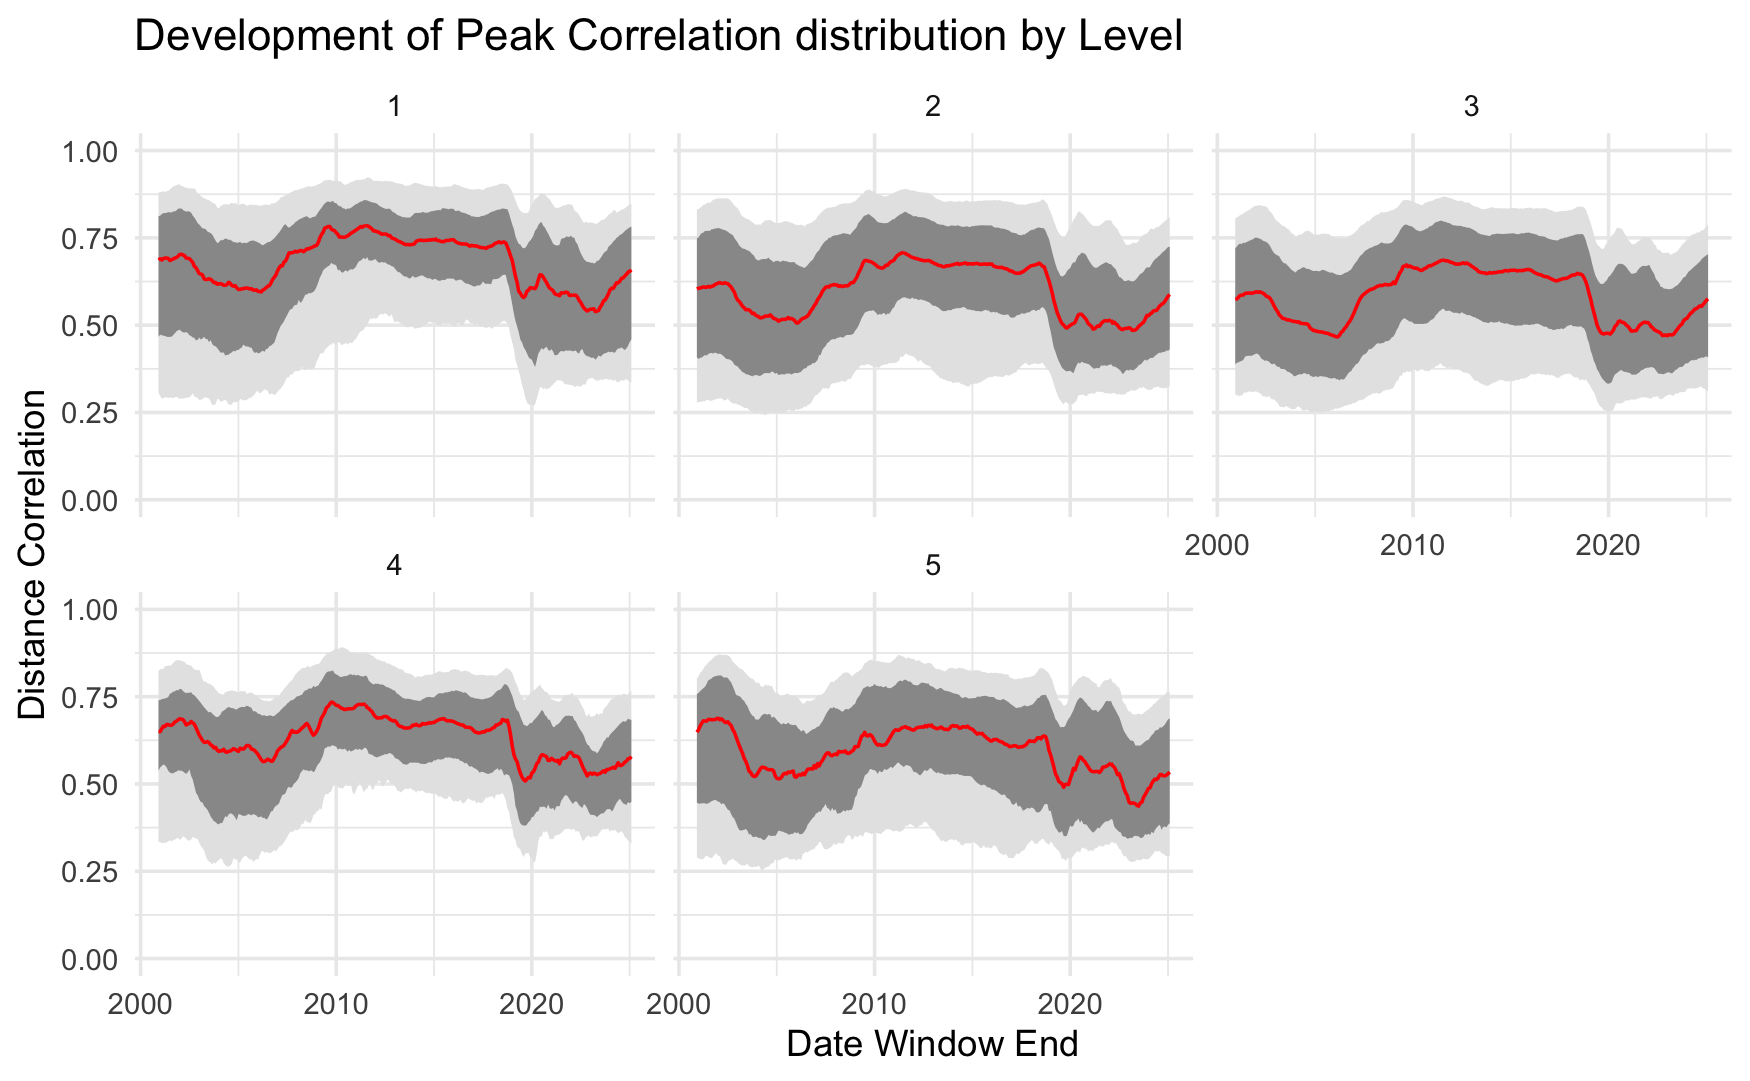
\includegraphics[width=0.7\linewidth]{DominikPlots/cd_dcor_dist_roll_level.png}
    \caption{Rolling-window distribution of peak distance correlations by level.}
    \label{fig:cd_dcor_dist_roll_level}
\end{figure}

From an analytical perspective, this is a noteworthy result. Because Levels~4--5 represent more disaggregated industries, their economic weight in the main index is much smaller than that of Level~1 or Level~2 sectors. Their alignment with the aggregate development is therefore not necessarily the result of construction, but likely reflects genuine causal links to overall business cycle dynamics. This suggests that lower-level industries may serve as a valuable indicative set for monitoring economic developments. Further investigation of these fine-grained series could thus provide useful insights into early signals of aggregate turning points.


\subsection{Consensus Analysis}
In the previous section we examined the variance of correlations across industries, which showed how strongly the dependence structure fluctuates over time. However, this analysis did not reveal whether the relative position of individual industries within the correlation structure remains stable or changes substantially. To address this, we introduce a ranking-based consensus analysis that evaluates the stability of industry rankings across time windows.

The idea is to compare, for each survey question and time window, the set of top-$k$ most strongly correlated industries.\footnote{Throughout the analysis we use $k=30$. This choice reflects a balance between capturing enough of the correlation structure and avoiding excessive noise from lower-ranked industries; robustness checks with alternative $k$ confirmed that the dynamics are well represented at this threshold.} By focusing on the overlap of these top-ranked industries, we can track whether the “core set” of highly correlated industries remains consistent or whether entirely new industries enter the picture over time.

To quantify this, we compute the Jaccard index between two sets $A$ and $B$ of top-$k$ industries:  
\[
  J(A,B) = \frac{|A \cap B|}{|A \cup B|} 
  = \frac{|A \cap B|}{2k - |A \cap B|},\footnote{The second equality holds only because both sets $A$ and $B$ are of equal size $k$. In the general case, the denominator is $|A \cup B|$ without simplification.}
\]
The Jaccard index ranges from $0$ (no overlap) to $1$ (perfect overlap), and thus measures how similar the top-$k$ sets are across windows. Averaging these pairwise values over time yields a nonlinear consensus metric that captures the overall stability of the ranking structure.

\begin{figure}[H]
    \centering
    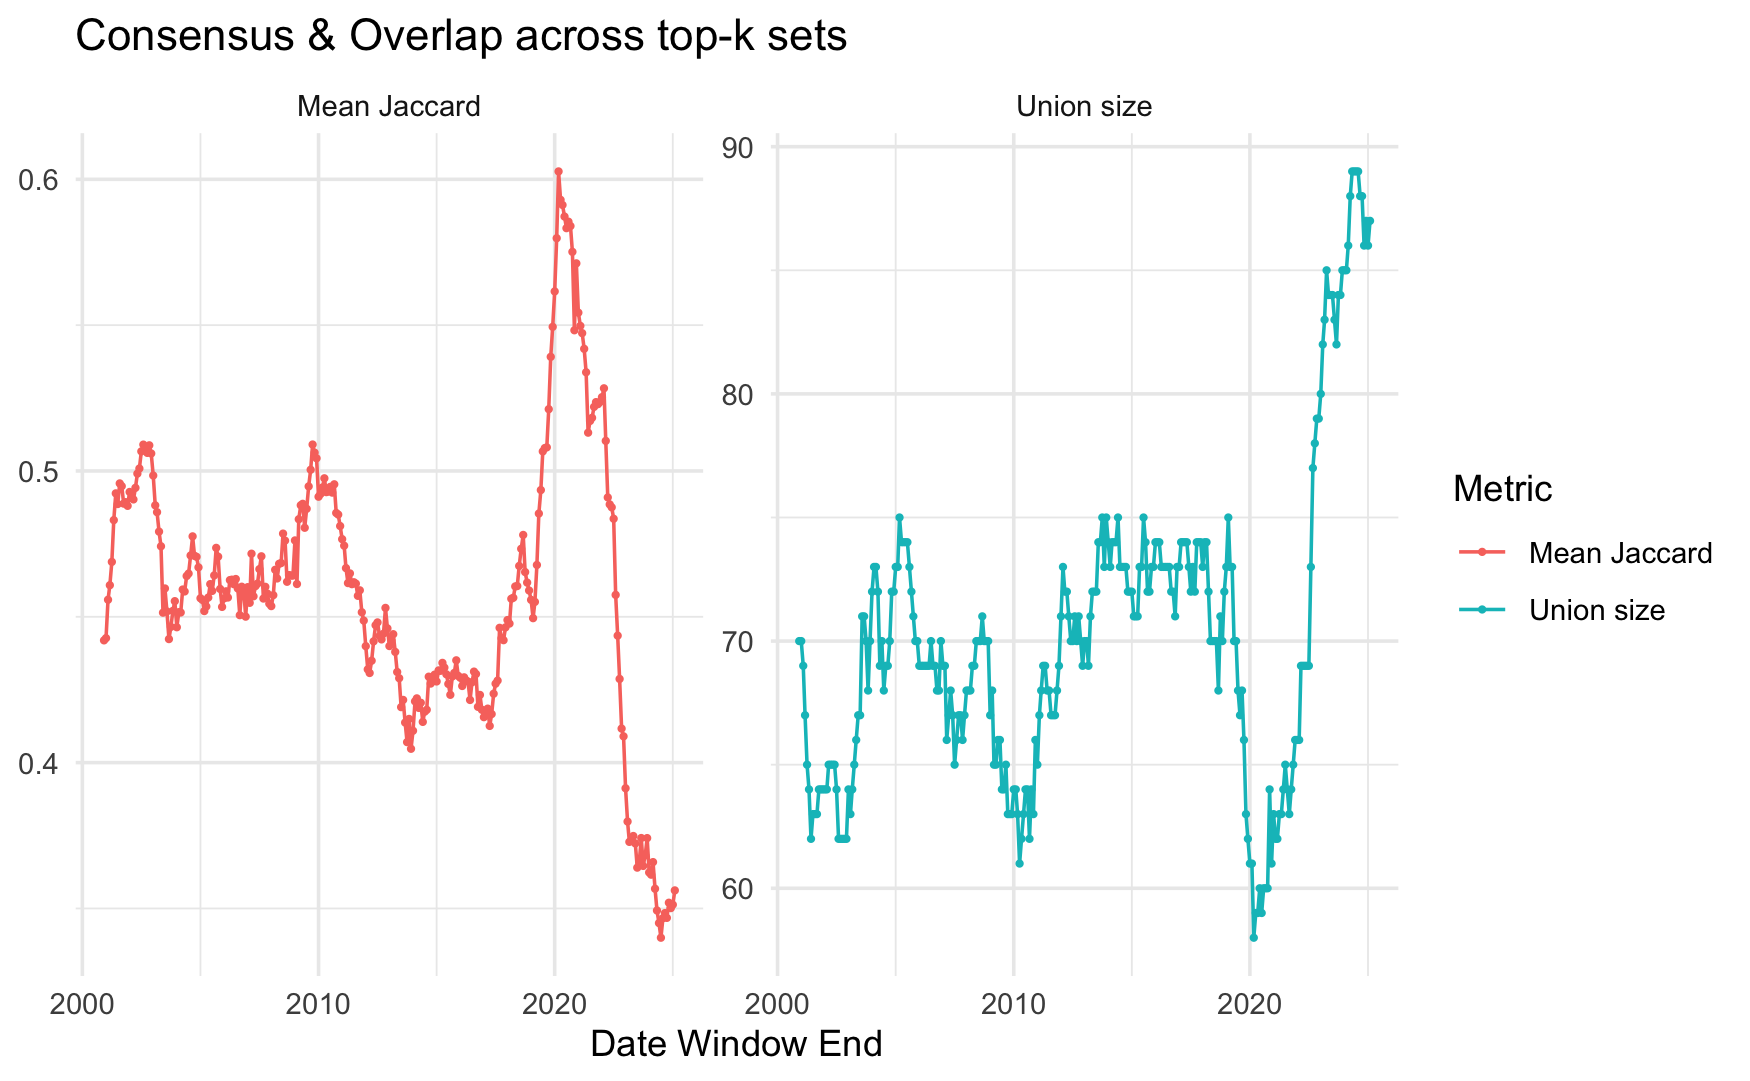
\includegraphics[width=0.7\linewidth]{DominikPlots/ca_jaccard_union.png}
    \caption{Consensus of top-30 sets (Jaccard index) vs.\ union size over time.}
\end{figure}

The results reveal two important features. First, higher average Jaccard values combined with smaller union sizes indicate that the structure is increasingly dominated by a relatively small group of industries, i.e., the same industries repeatedly occupy the top ranks. Second, we observe sharp spikes in consensus around major economic events. The strongest such spike occurs in 2020 during the COVID-19 pandemic, exceeding those seen during earlier crises such as the dot-com downturn in 2002 or the global financial crisis in 2008–2010. This pattern suggests that systemic shocks compress the correlation structure, temporarily aligning industries more closely than in normal times.

From an economic perspective, this alignment provides valuable information: during crises, the set of industries that best track the main index becomes more homogeneous, while in stable periods the ranking is more dispersed. In other words, systemic stress appears to “synchronize” industry-level dynamics. This observation points to the potential of consensus analysis as a diagnostic tool: sharp increases in consensus may serve as early signals of widespread economic stress. Further research should investigate whether such consensus spikes can be systematically linked to the onset of recessions or other structural breaks.

%---------------